\documentclass[1p]{elsarticle_modified}
%\bibliographystyle{elsarticle-num}

%\usepackage[colorlinks]{hyperref}
%\usepackage{abbrmath_seonhwa} %\Abb, \Ascr, \Acal ,\Abf, \Afrak
\usepackage{amsfonts}
\usepackage{amssymb}
\usepackage{amsmath}
\usepackage{amsthm}
\usepackage{scalefnt}
\usepackage{amsbsy}
\usepackage{kotex}
\usepackage{caption}
\usepackage{subfig}
\usepackage{color}
\usepackage{graphicx}
\usepackage{xcolor} %% white, black, red, green, blue, cyan, magenta, yellow
\usepackage{float}
\usepackage{setspace}
\usepackage{hyperref}

\usepackage{tikz}
\usetikzlibrary{arrows}

\usepackage{multirow}
\usepackage{array} % fixed length table
\usepackage{hhline}

%%%%%%%%%%%%%%%%%%%%%
\makeatletter
\renewcommand*\env@matrix[1][\arraystretch]{%
	\edef\arraystretch{#1}%
	\hskip -\arraycolsep
	\let\@ifnextchar\new@ifnextchar
	\array{*\c@MaxMatrixCols c}}
\makeatother %https://tex.stackexchange.com/questions/14071/how-can-i-increase-the-line-spacing-in-a-matrix
%%%%%%%%%%%%%%%

\usepackage[normalem]{ulem}

\newcommand{\msout}[1]{\ifmmode\text{\sout{\ensuremath{#1}}}\else\sout{#1}\fi}
%SOURCE: \msout is \stkout macro in https://tex.stackexchange.com/questions/20609/strikeout-in-math-mode

\newcommand{\cancel}[1]{
	\ifmmode
	{\color{red}\msout{#1}}
	\else
	{\color{red}\sout{#1}}
	\fi
}

\newcommand{\add}[1]{
	{\color{blue}\uwave{#1}}
}

\newcommand{\replace}[2]{
	\ifmmode
	{\color{red}\msout{#1}}{\color{blue}\uwave{#2}}
	\else
	{\color{red}\sout{#1}}{\color{blue}\uwave{#2}}
	\fi
}

\newcommand{\Sol}{\mathcal{S}} %segment
\newcommand{\D}{D} %diagram
\newcommand{\A}{\mathcal{A}} %arc


%%%%%%%%%%%%%%%%%%%%%%%%%%%%%5 test

\def\sl{\operatorname{\textup{SL}}(2,\Cbb)}
\def\psl{\operatorname{\textup{PSL}}(2,\Cbb)}
\def\quan{\mkern 1mu \triangleright \mkern 1mu}

\theoremstyle{definition}
\newtheorem{thm}{Theorem}[section]
\newtheorem{prop}[thm]{Proposition}
\newtheorem{lem}[thm]{Lemma}
\newtheorem{ques}[thm]{Question}
\newtheorem{cor}[thm]{Corollary}
\newtheorem{defn}[thm]{Definition}
\newtheorem{exam}[thm]{Example}
\newtheorem{rmk}[thm]{Remark}
\newtheorem{alg}[thm]{Algorithm}

\newcommand{\I}{\sqrt{-1}}
\begin{document}

%\begin{frontmatter}
%
%\title{Boundary parabolic representations of knots up to 8 crossings}
%
%%% Group authors per affiliation:
%\author{Yunhi Cho} 
%\address{Department of Mathematics, University of Seoul, Seoul, Korea}
%\ead{yhcho@uos.ac.kr}
%
%
%\author{Seonhwa Kim} %\fnref{s_kim}}
%\address{Center for Geometry and Physics, Institute for Basic Science, Pohang, 37673, Korea}
%\ead{ryeona17@ibs.re.kr}
%
%\author{Hyuk Kim}
%\address{Department of Mathematical Sciences, Seoul National University, Seoul 08826, Korea}
%\ead{hyukkim@snu.ac.kr}
%
%\author{Seokbeom Yoon}
%\address{Department of Mathematical Sciences, Seoul National University, Seoul, 08826,  Korea}
%\ead{sbyoon15@snu.ac.kr}
%
%\begin{abstract}
%We find all boundary parabolic representation of knots up to 8 crossings.
%
%\end{abstract}
%\begin{keyword}
%    \MSC[2010] 57M25 
%\end{keyword}
%
%\end{frontmatter}

%\linenumbers
%\tableofcontents
%
\newcommand\colored[1]{\textcolor{white}{\rule[-0.35ex]{0.8em}{1.4ex}}\kern-0.8em\color{red} #1}%
%\newcommand\colored[1]{\textcolor{white}{ #1}\kern-2.17ex	\textcolor{white}{ #1}\kern-1.81ex	\textcolor{white}{ #1}\kern-2.15ex\color{red}#1	}

{\Large $\underline{11a_{163}~(K11a_{163})}$}

\setlength{\tabcolsep}{10pt}
\renewcommand{\arraystretch}{1.6}
\vspace{1cm}\begin{tabular}{m{100pt}>{\centering\arraybackslash}m{274pt}}
\multirow{5}{120pt}{
	\centering
	\includegraphics[width=112pt]{../../../GIT/diagram.site/Diagrams/png/412_11a_163.png}\\
\ \ \ A knot diagram\footnotemark}&
\allowdisplaybreaks
\textbf{Linearized knot diagam} \\
\cline{2-2}
 &
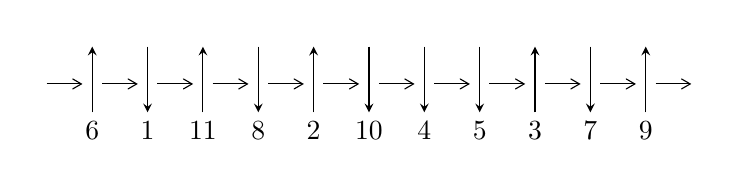
\begin{tikzpicture}[x=20pt, y=17pt]
	% nodes
	\node (C0) at (0, 0) {};
	\node (C1) at (1, 0) {};
	\node (C1U) at (1, +1) {};
	\node (C1D) at (1, -1) {6};

	\node (C2) at (2, 0) {};
	\node (C2U) at (2, +1) {};
	\node (C2D) at (2, -1) {1};

	\node (C3) at (3, 0) {};
	\node (C3U) at (3, +1) {};
	\node (C3D) at (3, -1) {11};

	\node (C4) at (4, 0) {};
	\node (C4U) at (4, +1) {};
	\node (C4D) at (4, -1) {8};

	\node (C5) at (5, 0) {};
	\node (C5U) at (5, +1) {};
	\node (C5D) at (5, -1) {2};

	\node (C6) at (6, 0) {};
	\node (C6U) at (6, +1) {};
	\node (C6D) at (6, -1) {10};

	\node (C7) at (7, 0) {};
	\node (C7U) at (7, +1) {};
	\node (C7D) at (7, -1) {4};

	\node (C8) at (8, 0) {};
	\node (C8U) at (8, +1) {};
	\node (C8D) at (8, -1) {5};

	\node (C9) at (9, 0) {};
	\node (C9U) at (9, +1) {};
	\node (C9D) at (9, -1) {3};

	\node (C10) at (10, 0) {};
	\node (C10U) at (10, +1) {};
	\node (C10D) at (10, -1) {7};

	\node (C11) at (11, 0) {};
	\node (C11U) at (11, +1) {};
	\node (C11D) at (11, -1) {9};
	\node (C12) at (12, 0) {};

	% arrows
	\draw[->,>={angle 60}]
	(C0) edge (C1) (C1) edge (C2) (C2) edge (C3) (C3) edge (C4) (C4) edge (C5) (C5) edge (C6) (C6) edge (C7) (C7) edge (C8) (C8) edge (C9) (C9) edge (C10) (C10) edge (C11) (C11) edge (C12) ;	\draw[->,>=stealth]
	(C1D) edge (C1U) (C2U) edge (C2D) (C3D) edge (C3U) (C4U) edge (C4D) (C5D) edge (C5U) (C6U) edge (C6D) (C7U) edge (C7D) (C8U) edge (C8D) (C9D) edge (C9U) (C10U) edge (C10D) (C11D) edge (C11U) ;
	\end{tikzpicture} \\
\hhline{~~} \\& 
\textbf{Solving Sequence} \\ \cline{2-2} 
 &
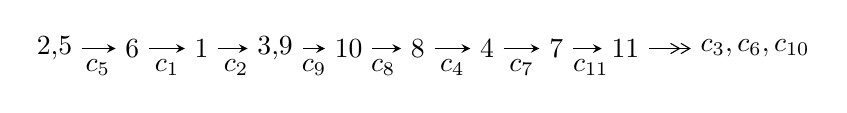
\begin{tikzpicture}[x=25pt, y=7pt]
	% node
	\node (A0) at (-1/8, 0) {2,5};
	\node (A1) at (1, 0) {6};
	\node (A2) at (2, 0) {1};
	\node (A3) at (49/16, 0) {3,9};
	\node (A4) at (33/8, 0) {10};
	\node (A5) at (41/8, 0) {8};
	\node (A6) at (49/8, 0) {4};
	\node (A7) at (57/8, 0) {7};
	\node (A8) at (65/8, 0) {11};
	\node (C1) at (1/2, -1) {$c_{5}$};
	\node (C2) at (3/2, -1) {$c_{1}$};
	\node (C3) at (5/2, -1) {$c_{2}$};
	\node (C4) at (29/8, -1) {$c_{9}$};
	\node (C5) at (37/8, -1) {$c_{8}$};
	\node (C6) at (45/8, -1) {$c_{4}$};
	\node (C7) at (53/8, -1) {$c_{7}$};
	\node (C8) at (61/8, -1) {$c_{11}$};
	\node (A9) at (10, 0) {$c_{3},c_{6},c_{10}$};

	% edge
	\draw[->,>=stealth]	
	(A0) edge (A1) (A1) edge (A2) (A2) edge (A3) (A3) edge (A4) (A4) edge (A5) (A5) edge (A6) (A6) edge (A7) (A7) edge (A8) ;
	\draw[->>,>={angle 60}]	
	(A8) edge (A9);
\end{tikzpicture} \\ 

\end{tabular} \\

\footnotetext{
The image of knot diagram is generated by the software ``\textbf{Draw programme}" developed by Andrew Bartholomew(\url{http://www.layer8.co.uk/maths/draw/index.htm\#Running-draw}), where we modified some parts for our purpose(\url{https://github.com/CATsTAILs/LinksPainter}).
}\phantom \\ \newline 
\centering \textbf{Ideals for irreducible components\footnotemark of $X_{\text{par}}$} 
 
\begin{align*}
I^u_{1}&=\langle 
3.66420\times10^{64} u^{71}-1.34364\times10^{65} u^{70}+\cdots+5.98806\times10^{65} b+5.69300\times10^{65},\\
\phantom{I^u_{1}}&\phantom{= \langle  }-1.86215\times10^{65} u^{71}+7.77862\times10^{65} u^{70}+\cdots+5.98806\times10^{65} a-1.33999\times10^{65},\;u^{72}+17 u^{70}+\cdots+u+1\rangle \\
I^u_{2}&=\langle 
2 u^{12}+u^{11}+6 u^{10}+3 u^9+11 u^8+7 u^7+7 u^6+10 u^5+8 u^3-3 u^2+b+2 u,\\
\phantom{I^u_{2}}&\phantom{= \langle  }u^{12}+u^{11}+3 u^{10}+2 u^9+4 u^8+2 u^7-4 u^4-2 u^3-3 u^2+a,\\
\phantom{I^u_{2}}&\phantom{= \langle  }u^{13}+u^{12}+4 u^{11}+3 u^{10}+8 u^9+6 u^8+8 u^7+7 u^6+3 u^5+6 u^4- u^3+3 u^2- u+1\rangle \\
\\
\end{align*}
\raggedright * 2 irreducible components of $\dim_{\mathbb{C}}=0$, with total 85 representations.\\
\footnotetext{All coefficients of polynomials are rational numbers. But the coefficients are sometimes approximated in decimal forms when there is not enough margin.}
\newpage
\renewcommand{\arraystretch}{1}
\centering \section*{I. $I^u_{1}= \langle 3.66\times10^{64} u^{71}-1.34\times10^{65} u^{70}+\cdots+5.99\times10^{65} b+5.69\times10^{65},\;-1.86\times10^{65} u^{71}+7.78\times10^{65} u^{70}+\cdots+5.99\times10^{65} a-1.34\times10^{65},\;u^{72}+17 u^{70}+\cdots+u+1 \rangle$}
\flushleft \textbf{(i) Arc colorings}\\
\begin{tabular}{m{7pt} m{180pt} m{7pt} m{180pt} }
\flushright $a_{2}=$&$\begin{pmatrix}0\\u\end{pmatrix}$ \\
\flushright $a_{5}=$&$\begin{pmatrix}1\\0\end{pmatrix}$ \\
\flushright $a_{6}=$&$\begin{pmatrix}1\\- u^2\end{pmatrix}$ \\
\flushright $a_{1}=$&$\begin{pmatrix}- u\\u^3+u\end{pmatrix}$ \\
\flushright $a_{3}=$&$\begin{pmatrix}- u^3\\u^5+u^3+u\end{pmatrix}$ \\
\flushright $a_{9}=$&$\begin{pmatrix}0.310978 u^{71}-1.29902 u^{70}+\cdots-3.70836 u+0.223776\\-0.0611917 u^{71}+0.224387 u^{70}+\cdots+1.02932 u-0.950725\end{pmatrix}$ \\
\flushright $a_{10}=$&$\begin{pmatrix}0.0969772 u^{71}-1.15579 u^{70}+\cdots-3.31741 u+0.426345\\-0.254667 u^{71}-0.194746 u^{70}+\cdots+0.186158 u-1.47703\end{pmatrix}$ \\
\flushright $a_{8}=$&$\begin{pmatrix}0.249786 u^{71}-1.07463 u^{70}+\cdots-2.67904 u-0.726949\\-0.0611917 u^{71}+0.224387 u^{70}+\cdots+1.02932 u-0.950725\end{pmatrix}$ \\
\flushright $a_{4}=$&$\begin{pmatrix}-2.35209 u^{71}-2.74506 u^{70}+\cdots-5.81147 u+0.452584\\-0.873645 u^{71}-0.690474 u^{70}+\cdots+0.140283 u-2.05357\end{pmatrix}$ \\
\flushright $a_{7}=$&$\begin{pmatrix}0.518603 u^{71}+1.42755 u^{70}+\cdots+7.61883 u+0.135936\\0.614017 u^{71}-0.318119 u^{70}+\cdots-1.29823 u+1.23094\end{pmatrix}$ \\
\flushright $a_{11}=$&$\begin{pmatrix}-1.75192 u^{71}-0.223371 u^{70}+\cdots-10.3144 u+0.548362\\-1.06712 u^{71}+0.982309 u^{70}+\cdots+4.11161 u+1.60445\end{pmatrix}$\\ \flushright $a_{11}=$&$\begin{pmatrix}-1.75192 u^{71}-0.223371 u^{70}+\cdots-10.3144 u+0.548362\\-1.06712 u^{71}+0.982309 u^{70}+\cdots+4.11161 u+1.60445\end{pmatrix}$\\&\end{tabular}
\flushleft \textbf{(ii) Obstruction class $= -1$}\\~\\
\flushleft \textbf{(iii) Cusp Shapes $= 1.46166 u^{71}-1.65225 u^{70}+\cdots-4.80947 u-8.48974$}\\~\\
\newpage\renewcommand{\arraystretch}{1}
\flushleft \textbf{(iv) u-Polynomials at the component}\newline \\
\begin{tabular}{m{50pt}|m{274pt}}
Crossings & \hspace{64pt}u-Polynomials at each crossing \\
\hline $$\begin{aligned}c_{1},c_{5}\end{aligned}$$&$\begin{aligned}
&u^{72}+17 u^{70}+\cdots+u+1
\end{aligned}$\\
\hline $$\begin{aligned}c_{2}\end{aligned}$$&$\begin{aligned}
&u^{72}+34 u^{71}+\cdots+11 u+1
\end{aligned}$\\
\hline $$\begin{aligned}c_{3}\end{aligned}$$&$\begin{aligned}
&u^{72}+6 u^{71}+\cdots+50529 u+18761
\end{aligned}$\\
\hline $$\begin{aligned}c_{4},c_{7},c_{8}\end{aligned}$$&$\begin{aligned}
&u^{72}+2 u^{71}+\cdots+17 u-1
\end{aligned}$\\
\hline $$\begin{aligned}c_{6},c_{10}\end{aligned}$$&$\begin{aligned}
&u^{72}- u^{71}+\cdots+704 u+121
\end{aligned}$\\
\hline $$\begin{aligned}c_{9}\end{aligned}$$&$\begin{aligned}
&u^{72}-2 u^{71}+\cdots-25 u-1
\end{aligned}$\\
\hline $$\begin{aligned}c_{11}\end{aligned}$$&$\begin{aligned}
&u^{72}+12 u^{71}+\cdots-916 u-88
\end{aligned}$\\
\hline
\end{tabular}\\~\\
\newpage\renewcommand{\arraystretch}{1}
\flushleft \textbf{(v) Riley Polynomials at the component}\newline \\
\begin{tabular}{m{50pt}|m{274pt}}
Crossings & \hspace{64pt}Riley Polynomials at each crossing \\
\hline $$\begin{aligned}c_{1},c_{5}\end{aligned}$$&$\begin{aligned}
&y^{72}+34 y^{71}+\cdots+11 y+1
\end{aligned}$\\
\hline $$\begin{aligned}c_{2}\end{aligned}$$&$\begin{aligned}
&y^{72}+14 y^{71}+\cdots+87 y+1
\end{aligned}$\\
\hline $$\begin{aligned}c_{3}\end{aligned}$$&$\begin{aligned}
&y^{72}+28 y^{71}+\cdots+9764167099 y+351975121
\end{aligned}$\\
\hline $$\begin{aligned}c_{4},c_{7},c_{8}\end{aligned}$$&$\begin{aligned}
&y^{72}-76 y^{71}+\cdots-13 y+1
\end{aligned}$\\
\hline $$\begin{aligned}c_{6},c_{10}\end{aligned}$$&$\begin{aligned}
&y^{72}-59 y^{71}+\cdots-471900 y+14641
\end{aligned}$\\
\hline $$\begin{aligned}c_{9}\end{aligned}$$&$\begin{aligned}
&y^{72}+4 y^{71}+\cdots-33 y+1
\end{aligned}$\\
\hline $$\begin{aligned}c_{11}\end{aligned}$$&$\begin{aligned}
&y^{72}+8 y^{71}+\cdots+92336 y+7744
\end{aligned}$\\
\hline
\end{tabular}\\~\\
\newpage\flushleft \textbf{(vi) Complex Volumes and Cusp Shapes}
$$\begin{array}{c|c|c}  
\text{Solutions to }I^u_{1}& \I (\text{vol} + \sqrt{-1}CS) & \text{Cusp shape}\\
 \hline 
\begin{aligned}
u &= -0.840708 + 0.557697 I \\
a &= -0.880577 - 0.427963 I \\
b &= \phantom{-}1.343390 - 0.024122 I\end{aligned}
 & -2.78766 - 0.58394 I & -2.05211 + 2.44149 I \\ \hline\begin{aligned}
u &= -0.840708 - 0.557697 I \\
a &= -0.880577 + 0.427963 I \\
b &= \phantom{-}1.343390 + 0.024122 I\end{aligned}
 & -2.78766 + 0.58394 I & -2.05211 - 2.44149 I \\ \hline\begin{aligned}
u &= \phantom{-}0.950154 + 0.340310 I \\
a &= \phantom{-}0.730739 + 0.652349 I \\
b &= -1.54739 - 0.27859 I\end{aligned}
 & -7.89489 - 10.18180 I & -4.39970 + 5.17085 I \\ \hline\begin{aligned}
u &= \phantom{-}0.950154 - 0.340310 I \\
a &= \phantom{-}0.730739 - 0.652349 I \\
b &= -1.54739 + 0.27859 I\end{aligned}
 & -7.89489 + 10.18180 I & -4.39970 - 5.17085 I \\ \hline\begin{aligned}
u &= -0.341711 + 0.959879 I \\
a &= -0.96938 + 2.00953 I \\
b &= -0.220351 + 0.064200 I\end{aligned}
 & -4.43635 - 1.24068 I & -13.95090 + 0. I\phantom{ +0.000000I} \\ \hline\begin{aligned}
u &= -0.341711 - 0.959879 I \\
a &= -0.96938 - 2.00953 I \\
b &= -0.220351 - 0.064200 I\end{aligned}
 & -4.43635 + 1.24068 I & -13.95090 + 0. I\phantom{ +0.000000I} \\ \hline\begin{aligned}
u &= \phantom{-}0.314455 + 0.987227 I \\
a &= -1.18996 - 1.25711 I \\
b &= -0.240890 + 1.025020 I\end{aligned}
 & -4.69737 + 1.04071 I & -11.41192 + 0. I\phantom{ +0.000000I} \\ \hline\begin{aligned}
u &= \phantom{-}0.314455 - 0.987227 I \\
a &= -1.18996 + 1.25711 I \\
b &= -0.240890 - 1.025020 I\end{aligned}
 & -4.69737 - 1.04071 I & -11.41192 + 0. I\phantom{ +0.000000I} \\ \hline\begin{aligned}
u &= \phantom{-}0.775035 + 0.705599 I \\
a &= \phantom{-}0.106869 + 0.795488 I \\
b &= \phantom{-}0.140516 - 0.628949 I\end{aligned}
 & \phantom{-}0.45501 + 2.74412 I & \phantom{-0.000000 } 0. - 6.58454 I \\ \hline\begin{aligned}
u &= \phantom{-}0.775035 - 0.705599 I \\
a &= \phantom{-}0.106869 - 0.795488 I \\
b &= \phantom{-}0.140516 + 0.628949 I\end{aligned}
 & \phantom{-}0.45501 - 2.74412 I & \phantom{-0.000000 -}0. + 6.58454 I\\
 \hline 
 \end{array}$$\newpage$$\begin{array}{c|c|c}  
\text{Solutions to }I^u_{1}& \I (\text{vol} + \sqrt{-1}CS) & \text{Cusp shape}\\
 \hline 
\begin{aligned}
u &= -1.05938\phantom{ +0.000000I} \\
a &= \phantom{-}0.181417\phantom{ +0.000000I} \\
b &= -1.41763\phantom{ +0.000000I}\end{aligned}
 & -3.29623\phantom{ +0.000000I} & -2.05430\phantom{ +0.000000I} \\ \hline\begin{aligned}
u &= \phantom{-}0.474907 + 0.952227 I \\
a &= -0.633361 - 0.443998 I \\
b &= \phantom{-}0.748919 + 0.467243 I\end{aligned}
 & -0.15843 + 2.64508 I & \phantom{-0.000000 } 0 \\ \hline\begin{aligned}
u &= \phantom{-}0.474907 - 0.952227 I \\
a &= -0.633361 + 0.443998 I \\
b &= \phantom{-}0.748919 - 0.467243 I\end{aligned}
 & -0.15843 - 2.64508 I & \phantom{-0.000000 } 0 \\ \hline\begin{aligned}
u &= \phantom{-}0.541899 + 0.922731 I \\
a &= \phantom{-}0.420914 + 0.880805 I \\
b &= \phantom{-}0.174435 - 0.624288 I\end{aligned}
 & \phantom{-}0.03676 + 2.24980 I & \phantom{-0.000000 } 0 \\ \hline\begin{aligned}
u &= \phantom{-}0.541899 - 0.922731 I \\
a &= \phantom{-}0.420914 - 0.880805 I \\
b &= \phantom{-}0.174435 + 0.624288 I\end{aligned}
 & \phantom{-}0.03676 - 2.24980 I & \phantom{-0.000000 } 0 \\ \hline\begin{aligned}
u &= -0.834732 + 0.404612 I \\
a &= -0.539302 + 1.118290 I \\
b &= \phantom{-}0.549489 - 0.813801 I\end{aligned}
 & -1.04725 + 6.18742 I & -1.76655 - 5.50914 I \\ \hline\begin{aligned}
u &= -0.834732 - 0.404612 I \\
a &= -0.539302 - 1.118290 I \\
b &= \phantom{-}0.549489 + 0.813801 I\end{aligned}
 & -1.04725 - 6.18742 I & -1.76655 + 5.50914 I \\ \hline\begin{aligned}
u &= \phantom{-}0.794162 + 0.453233 I \\
a &= -1.084850 - 0.732074 I \\
b &= \phantom{-}1.44309 + 0.14451 I\end{aligned}
 & -3.22516 - 3.95142 I & -2.96229 + 3.51289 I \\ \hline\begin{aligned}
u &= \phantom{-}0.794162 - 0.453233 I \\
a &= -1.084850 + 0.732074 I \\
b &= \phantom{-}1.44309 - 0.14451 I\end{aligned}
 & -3.22516 + 3.95142 I & -2.96229 - 3.51289 I \\ \hline\begin{aligned}
u &= -0.005532 + 1.088180 I \\
a &= -1.073720 + 0.449198 I \\
b &= -1.53636 - 0.04905 I\end{aligned}
 & -8.67044 - 2.20266 I & -8.24814 + 0. I\phantom{ +0.000000I}\\
 \hline 
 \end{array}$$\newpage$$\begin{array}{c|c|c}  
\text{Solutions to }I^u_{1}& \I (\text{vol} + \sqrt{-1}CS) & \text{Cusp shape}\\
 \hline 
\begin{aligned}
u &= -0.005532 - 1.088180 I \\
a &= -1.073720 - 0.449198 I \\
b &= -1.53636 + 0.04905 I\end{aligned}
 & -8.67044 + 2.20266 I & -8.24814 + 0. I\phantom{ +0.000000I} \\ \hline\begin{aligned}
u &= \phantom{-}0.426028 + 1.029620 I \\
a &= \phantom{-}2.09550 + 0.82862 I \\
b &= \phantom{-}1.56968 - 0.04690 I\end{aligned}
 & -10.60600 + 5.33661 I & \phantom{-0.000000 } 0 \\ \hline\begin{aligned}
u &= \phantom{-}0.426028 - 1.029620 I \\
a &= \phantom{-}2.09550 - 0.82862 I \\
b &= \phantom{-}1.56968 + 0.04690 I\end{aligned}
 & -10.60600 - 5.33661 I & \phantom{-0.000000 } 0 \\ \hline\begin{aligned}
u &= -0.880421\phantom{ +0.000000I} \\
a &= -0.281963\phantom{ +0.000000I} \\
b &= \phantom{-}1.12632\phantom{ +0.000000I}\end{aligned}
 & -1.79480\phantom{ +0.000000I} & -8.89990\phantom{ +0.000000I} \\ \hline\begin{aligned}
u &= -0.421636 + 1.054610 I \\
a &= \phantom{-}0.447812 - 0.783280 I \\
b &= \phantom{-}1.69289 - 0.25084 I\end{aligned}
 & -11.08040 - 0.40194 I & \phantom{-0.000000 } 0 \\ \hline\begin{aligned}
u &= -0.421636 - 1.054610 I \\
a &= \phantom{-}0.447812 + 0.783280 I \\
b &= \phantom{-}1.69289 + 0.25084 I\end{aligned}
 & -11.08040 + 0.40194 I & \phantom{-0.000000 } 0 \\ \hline\begin{aligned}
u &= \phantom{-}0.470200 + 1.042550 I \\
a &= \phantom{-}0.79513 + 2.99296 I \\
b &= \phantom{-}1.47270 - 0.0001 I\end{aligned}
 & -10.28460 + 1.13066 I & \phantom{-0.000000 } 0 \\ \hline\begin{aligned}
u &= \phantom{-}0.470200 - 1.042550 I \\
a &= \phantom{-}0.79513 - 2.99296 I \\
b &= \phantom{-}1.47270 + 0.0001 I\end{aligned}
 & -10.28460 - 1.13066 I & \phantom{-0.000000 } 0 \\ \hline\begin{aligned}
u &= -0.533946 + 1.013710 I \\
a &= -0.879687 + 0.301042 I \\
b &= -0.662168 - 0.098832 I\end{aligned}
 & -3.06053 - 4.69031 I & \phantom{-0.000000 } 0 \\ \hline\begin{aligned}
u &= -0.533946 - 1.013710 I \\
a &= -0.879687 - 0.301042 I \\
b &= -0.662168 + 0.098832 I\end{aligned}
 & -3.06053 + 4.69031 I & \phantom{-0.000000 } 0\\
 \hline 
 \end{array}$$\newpage$$\begin{array}{c|c|c}  
\text{Solutions to }I^u_{1}& \I (\text{vol} + \sqrt{-1}CS) & \text{Cusp shape}\\
 \hline 
\begin{aligned}
u &= -0.208920 + 0.825464 I \\
a &= \phantom{-}0.353262 + 0.439079 I \\
b &= \phantom{-}0.594004 - 0.357212 I\end{aligned}
 & -1.46471 + 0.85730 I & -6.08976 - 4.46736 I \\ \hline\begin{aligned}
u &= -0.208920 - 0.825464 I \\
a &= \phantom{-}0.353262 - 0.439079 I \\
b &= \phantom{-}0.594004 + 0.357212 I\end{aligned}
 & -1.46471 - 0.85730 I & -6.08976 + 4.46736 I \\ \hline\begin{aligned}
u &= \phantom{-}0.442925 + 0.726814 I \\
a &= -0.30006 - 2.18686 I \\
b &= -0.947495 + 0.274305 I\end{aligned}
 & \phantom{-}0.609165 + 1.192600 I & -2.86974 - 6.15662 I \\ \hline\begin{aligned}
u &= \phantom{-}0.442925 - 0.726814 I \\
a &= -0.30006 + 2.18686 I \\
b &= -0.947495 - 0.274305 I\end{aligned}
 & \phantom{-}0.609165 - 1.192600 I & -2.86974 + 6.15662 I \\ \hline\begin{aligned}
u &= -0.462289 + 1.065050 I \\
a &= \phantom{-}0.35283 - 2.29105 I \\
b &= \phantom{-}1.57534 + 0.38822 I\end{aligned}
 & -10.78700 - 6.40801 I & \phantom{-0.000000 } 0 \\ \hline\begin{aligned}
u &= -0.462289 - 1.065050 I \\
a &= \phantom{-}0.35283 + 2.29105 I \\
b &= \phantom{-}1.57534 - 0.38822 I\end{aligned}
 & -10.78700 + 6.40801 I & \phantom{-0.000000 } 0 \\ \hline\begin{aligned}
u &= -0.651335 + 0.521113 I \\
a &= \phantom{-}0.60688 - 1.32770 I \\
b &= -0.286712 + 0.512099 I\end{aligned}
 & \phantom{-}2.41607 + 1.66211 I & \phantom{-}3.86075 - 3.01699 I \\ \hline\begin{aligned}
u &= -0.651335 - 0.521113 I \\
a &= \phantom{-}0.60688 + 1.32770 I \\
b &= -0.286712 - 0.512099 I\end{aligned}
 & \phantom{-}2.41607 - 1.66211 I & \phantom{-}3.86075 + 3.01699 I \\ \hline\begin{aligned}
u &= -0.575499 + 1.031320 I \\
a &= \phantom{-}0.47397 - 1.46431 I \\
b &= \phantom{-}0.371678 + 0.605414 I\end{aligned}
 & \phantom{-}0.91167 - 6.46667 I & \phantom{-0.000000 } 0 \\ \hline\begin{aligned}
u &= -0.575499 - 1.031320 I \\
a &= \phantom{-}0.47397 + 1.46431 I \\
b &= \phantom{-}0.371678 - 0.605414 I\end{aligned}
 & \phantom{-}0.91167 + 6.46667 I & \phantom{-0.000000 } 0\\
 \hline 
 \end{array}$$\newpage$$\begin{array}{c|c|c}  
\text{Solutions to }I^u_{1}& \I (\text{vol} + \sqrt{-1}CS) & \text{Cusp shape}\\
 \hline 
\begin{aligned}
u &= \phantom{-}0.550811 + 1.056740 I \\
a &= \phantom{-}0.747495 + 0.338296 I \\
b &= -0.639979 - 1.016950 I\end{aligned}
 & -2.99967 + 5.33296 I & \phantom{-0.000000 } 0 \\ \hline\begin{aligned}
u &= \phantom{-}0.550811 - 1.056740 I \\
a &= \phantom{-}0.747495 - 0.338296 I \\
b &= -0.639979 + 1.016950 I\end{aligned}
 & -2.99967 - 5.33296 I & \phantom{-0.000000 } 0 \\ \hline\begin{aligned}
u &= -0.086155 + 1.193610 I \\
a &= -0.013978 + 0.141660 I \\
b &= -0.653821 + 0.551694 I\end{aligned}
 & -6.57891 + 3.67515 I & \phantom{-0.000000 } 0 \\ \hline\begin{aligned}
u &= -0.086155 - 1.193610 I \\
a &= -0.013978 - 0.141660 I \\
b &= -0.653821 - 0.551694 I\end{aligned}
 & -6.57891 - 3.67515 I & \phantom{-0.000000 } 0 \\ \hline\begin{aligned}
u &= \phantom{-}0.614768 + 0.453497 I \\
a &= \phantom{-}0.21295 + 1.65927 I \\
b &= \phantom{-}0.649805 - 0.820980 I\end{aligned}
 & -1.24059 - 0.70092 I & -3.96458 + 1.25636 I \\ \hline\begin{aligned}
u &= \phantom{-}0.614768 - 0.453497 I \\
a &= \phantom{-}0.21295 - 1.65927 I \\
b &= \phantom{-}0.649805 + 0.820980 I\end{aligned}
 & -1.24059 + 0.70092 I & -3.96458 - 1.25636 I \\ \hline\begin{aligned}
u &= \phantom{-}0.613054 + 1.092110 I \\
a &= -0.09290 - 2.30276 I \\
b &= -1.47613 + 0.18050 I\end{aligned}
 & -5.13451 + 9.23572 I & \phantom{-0.000000 } 0 \\ \hline\begin{aligned}
u &= \phantom{-}0.613054 - 1.092110 I \\
a &= -0.09290 + 2.30276 I \\
b &= -1.47613 - 0.18050 I\end{aligned}
 & -5.13451 - 9.23572 I & \phantom{-0.000000 } 0 \\ \hline\begin{aligned}
u &= -0.614621 + 1.121980 I \\
a &= -0.68974 + 1.30969 I \\
b &= -0.638676 - 0.884132 I\end{aligned}
 & -3.19452 - 11.57250 I & \phantom{-0.000000 } 0 \\ \hline\begin{aligned}
u &= -0.614621 - 1.121980 I \\
a &= -0.68974 - 1.30969 I \\
b &= -0.638676 + 0.884132 I\end{aligned}
 & -3.19452 + 11.57250 I & \phantom{-0.000000 } 0\\
 \hline 
 \end{array}$$\newpage$$\begin{array}{c|c|c}  
\text{Solutions to }I^u_{1}& \I (\text{vol} + \sqrt{-1}CS) & \text{Cusp shape}\\
 \hline 
\begin{aligned}
u &= \phantom{-}0.681999 + 0.181568 I \\
a &= \phantom{-}0.673913 - 0.420450 I \\
b &= -0.081091 + 0.148188 I\end{aligned}
 & \phantom{-}1.48009 + 0.06732 I & \phantom{-}8.50693 + 1.19475 I \\ \hline\begin{aligned}
u &= \phantom{-}0.681999 - 0.181568 I \\
a &= \phantom{-}0.673913 + 0.420450 I \\
b &= -0.081091 - 0.148188 I\end{aligned}
 & \phantom{-}1.48009 - 0.06732 I & \phantom{-}8.50693 - 1.19475 I \\ \hline\begin{aligned}
u &= -0.838953 + 0.988789 I \\
a &= \phantom{-}0.222398 + 0.901799 I \\
b &= -1.346560 - 0.145983 I\end{aligned}
 & -4.06336 - 5.47241 I & \phantom{-0.000000 } 0 \\ \hline\begin{aligned}
u &= -0.838953 - 0.988789 I \\
a &= \phantom{-}0.222398 - 0.901799 I \\
b &= -1.346560 + 0.145983 I\end{aligned}
 & -4.06336 + 5.47241 I & \phantom{-0.000000 } 0 \\ \hline\begin{aligned}
u &= \phantom{-}0.079295 + 0.696769 I \\
a &= -1.44779 + 1.05434 I \\
b &= -1.58629 - 0.11135 I\end{aligned}
 & -8.96742 - 2.37559 I & -5.52309 + 3.97031 I \\ \hline\begin{aligned}
u &= \phantom{-}0.079295 - 0.696769 I \\
a &= -1.44779 - 1.05434 I \\
b &= -1.58629 + 0.11135 I\end{aligned}
 & -8.96742 + 2.37559 I & -5.52309 - 3.97031 I \\ \hline\begin{aligned}
u &= -0.609332 + 1.155210 I \\
a &= -0.38230 + 1.37330 I \\
b &= -1.360490 - 0.234606 I\end{aligned}
 & -4.80243 - 5.41014 I & \phantom{-0.000000 } 0 \\ \hline\begin{aligned}
u &= -0.609332 - 1.155210 I \\
a &= -0.38230 - 1.37330 I \\
b &= -1.360490 + 0.234606 I\end{aligned}
 & -4.80243 + 5.41014 I & \phantom{-0.000000 } 0 \\ \hline\begin{aligned}
u &= \phantom{-}0.600309 + 1.184400 I \\
a &= -0.265300 - 0.552477 I \\
b &= -0.248151 + 0.167852 I\end{aligned}
 & -1.42281 + 5.04884 I & \phantom{-0.000000 } 0 \\ \hline\begin{aligned}
u &= \phantom{-}0.600309 - 1.184400 I \\
a &= -0.265300 + 0.552477 I \\
b &= -0.248151 - 0.167852 I\end{aligned}
 & -1.42281 - 5.04884 I & \phantom{-0.000000 } 0\\
 \hline 
 \end{array}$$\newpage$$\begin{array}{c|c|c}  
\text{Solutions to }I^u_{1}& \I (\text{vol} + \sqrt{-1}CS) & \text{Cusp shape}\\
 \hline 
\begin{aligned}
u &= \phantom{-}0.630641 + 1.185250 I \\
a &= \phantom{-}0.45048 + 1.91943 I \\
b &= \phantom{-}1.58800 - 0.29668 I\end{aligned}
 & -10.4703 + 15.9193 I & \phantom{-0.000000 } 0 \\ \hline\begin{aligned}
u &= \phantom{-}0.630641 - 1.185250 I \\
a &= \phantom{-}0.45048 - 1.91943 I \\
b &= \phantom{-}1.58800 + 0.29668 I\end{aligned}
 & -10.4703 - 15.9193 I & \phantom{-0.000000 } 0 \\ \hline\begin{aligned}
u &= \phantom{-}0.157141 + 1.357400 I \\
a &= \phantom{-}0.921605 + 0.073306 I \\
b &= \phantom{-}1.55044 + 0.19302 I\end{aligned}
 & -13.8147 - 6.4968 I & \phantom{-0.000000 } 0 \\ \hline\begin{aligned}
u &= \phantom{-}0.157141 - 1.357400 I \\
a &= \phantom{-}0.921605 - 0.073306 I \\
b &= \phantom{-}1.55044 - 0.19302 I\end{aligned}
 & -13.8147 + 6.4968 I & \phantom{-0.000000 } 0 \\ \hline\begin{aligned}
u &= -0.482865 + 0.381048 I \\
a &= \phantom{-}0.522791 + 0.286679 I \\
b &= \phantom{-}0.647093 - 0.330038 I\end{aligned}
 & -1.50033 + 0.49934 I & -4.97310 - 1.55605 I \\ \hline\begin{aligned}
u &= -0.482865 - 0.381048 I \\
a &= \phantom{-}0.522791 - 0.286679 I \\
b &= \phantom{-}0.647093 + 0.330038 I\end{aligned}
 & -1.50033 - 0.49934 I & -4.97310 + 1.55605 I \\ \hline\begin{aligned}
u &= -0.59705 + 1.31039 I \\
a &= \phantom{-}0.650728 - 1.145870 I \\
b &= \phantom{-}1.46461 + 0.05246 I\end{aligned}
 & -7.22620 - 5.83293 I & \phantom{-0.000000 } 0 \\ \hline\begin{aligned}
u &= -0.59705 - 1.31039 I \\
a &= \phantom{-}0.650728 + 1.145870 I \\
b &= \phantom{-}1.46461 - 0.05246 I\end{aligned}
 & -7.22620 + 5.83293 I & \phantom{-0.000000 } 0 \\ \hline\begin{aligned}
u &= \phantom{-}0.293343 + 0.413513 I \\
a &= \phantom{-}2.10950 + 1.82789 I \\
b &= -1.44649 + 0.12482 I\end{aligned}
 & -8.45650 + 2.58799 I & -6.38429 - 2.67811 I \\ \hline\begin{aligned}
u &= \phantom{-}0.293343 - 0.413513 I \\
a &= \phantom{-}2.10950 - 1.82789 I \\
b &= -1.44649 - 0.12482 I\end{aligned}
 & -8.45650 - 2.58799 I & -6.38429 + 2.67811 I\\
 \hline 
 \end{array}$$\newpage$$\begin{array}{c|c|c}  
\text{Solutions to }I^u_{1}& \I (\text{vol} + \sqrt{-1}CS) & \text{Cusp shape}\\
 \hline 
\begin{aligned}
u &= -0.335948 + 0.212346 I \\
a &= \phantom{-}3.09741 - 1.06498 I \\
b &= -1.51139 + 0.23154 I\end{aligned}
 & -8.60610 + 2.68144 I & -5.49009 - 1.95050 I \\ \hline\begin{aligned}
u &= -0.335948 - 0.212346 I \\
a &= \phantom{-}3.09741 + 1.06498 I \\
b &= -1.51139 - 0.23154 I\end{aligned}
 & -8.60610 - 2.68144 I & -5.49009 + 1.95050 I\\
 \hline 
 \end{array}$$\newpage\newpage\renewcommand{\arraystretch}{1}
\centering \section*{II. $I^u_{2}= \langle 2 u^{12}+u^{11}+\cdots+b+2 u,\;u^{12}+u^{11}+\cdots-3 u^2+a,\;u^{13}+u^{12}+\cdots- u+1 \rangle$}
\flushleft \textbf{(i) Arc colorings}\\
\begin{tabular}{m{7pt} m{180pt} m{7pt} m{180pt} }
\flushright $a_{2}=$&$\begin{pmatrix}0\\u\end{pmatrix}$ \\
\flushright $a_{5}=$&$\begin{pmatrix}1\\0\end{pmatrix}$ \\
\flushright $a_{6}=$&$\begin{pmatrix}1\\- u^2\end{pmatrix}$ \\
\flushright $a_{1}=$&$\begin{pmatrix}- u\\u^3+u\end{pmatrix}$ \\
\flushright $a_{3}=$&$\begin{pmatrix}- u^3\\u^5+u^3+u\end{pmatrix}$ \\
\flushright $a_{9}=$&$\begin{pmatrix}- u^{12}- u^{11}-3 u^{10}-2 u^9-4 u^8-2 u^7+4 u^4+2 u^3+3 u^2\\-2 u^{12}- u^{11}-6 u^{10}-3 u^9-11 u^8-7 u^7-7 u^6-10 u^5-8 u^3+3 u^2-2 u\end{pmatrix}$ \\
\flushright $a_{10}=$&$\begin{pmatrix}- u^{12}- u^{11}-3 u^{10}-3 u^9-5 u^8-5 u^7-2 u^6-4 u^5+u^4+u^3+u^2+u-1\\-2 u^{12}- u^{11}-6 u^{10}-3 u^9-11 u^8-7 u^7-7 u^6-10 u^5-7 u^3+3 u^2- u\end{pmatrix}$ \\
\flushright $a_{8}=$&$\begin{pmatrix}-3 u^{12}-2 u^{11}+\cdots+6 u^2-2 u\\-2 u^{12}- u^{11}-6 u^{10}-3 u^9-11 u^8-7 u^7-7 u^6-10 u^5-8 u^3+3 u^2-2 u\end{pmatrix}$ \\
\flushright $a_{4}=$&$\begin{pmatrix}u^{12}+u^{11}+2 u^{10}+2 u^9+2 u^8+3 u^7-2 u^6+u^5-2 u^4-3 u^3+u^2-2 u+1\\- u^{12}- u^{11}-3 u^{10}-2 u^9-5 u^8-4 u^7-3 u^6-3 u^5-3 u^3+u^2-1\end{pmatrix}$ \\
\flushright $a_{7}=$&$\begin{pmatrix}2 u^{12}+4 u^{10}- u^9+6 u^8- u^6+4 u^5-4 u^4+6 u^3-3 u^2+2 u\\3 u^{12}+2 u^{11}+\cdots+2 u+1\end{pmatrix}$ \\
\flushright $a_{11}=$&$\begin{pmatrix}3 u^{12}+2 u^{11}+\cdots-3 u^2+4 u\\u^{12}+u^{11}+3 u^{10}+3 u^9+5 u^8+6 u^7+3 u^6+6 u^5+u^4+3 u^3+2 u^2- u+2\end{pmatrix}$\\ \flushright $a_{11}=$&$\begin{pmatrix}3 u^{12}+2 u^{11}+\cdots-3 u^2+4 u\\u^{12}+u^{11}+3 u^{10}+3 u^9+5 u^8+6 u^7+3 u^6+6 u^5+u^4+3 u^3+2 u^2- u+2\end{pmatrix}$\\&\end{tabular}
\flushleft \textbf{(ii) Obstruction class $= 1$}\\~\\
\flushleft \textbf{(iii) Cusp Shapes $= -6 u^{12}-6 u^{11}-20 u^{10}-13 u^9-33 u^8-24 u^7-21 u^6-22 u^5+6 u^4-20 u^3+10 u^2-5 u-3$}\\~\\
\newpage\renewcommand{\arraystretch}{1}
\flushleft \textbf{(iv) u-Polynomials at the component}\newline \\
\begin{tabular}{m{50pt}|m{274pt}}
Crossings & \hspace{64pt}u-Polynomials at each crossing \\
\hline $$\begin{aligned}c_{1}\end{aligned}$$&$\begin{aligned}
&u^{13}- u^{12}+\cdots- u-1
\end{aligned}$\\
\hline $$\begin{aligned}c_{2}\end{aligned}$$&$\begin{aligned}
&u^{13}+7 u^{12}+\cdots-5 u-1
\end{aligned}$\\
\hline $$\begin{aligned}c_{3}\end{aligned}$$&$\begin{aligned}
&u^{13}+u^{12}- u^{11}-5 u^{10}-2 u^9+u^8+u^7- u^6+3 u^5+3 u^4+u^3- u^2- u-1
\end{aligned}$\\
\hline $$\begin{aligned}c_{4}\end{aligned}$$&$\begin{aligned}
&u^{13}+u^{12}+\cdots- u-1
\end{aligned}$\\
\hline $$\begin{aligned}c_{5}\end{aligned}$$&$\begin{aligned}
&u^{13}+u^{12}+\cdots- u+1
\end{aligned}$\\
\hline $$\begin{aligned}c_{6}\end{aligned}$$&$\begin{aligned}
&u^{13}+2 u^{12}+\cdots-7 u^2+1
\end{aligned}$\\
\hline $$\begin{aligned}c_{7},c_{8}\end{aligned}$$&$\begin{aligned}
&u^{13}- u^{12}+\cdots- u+1
\end{aligned}$\\
\hline $$\begin{aligned}c_{9}\end{aligned}$$&$\begin{aligned}
&u^{13}- u^{12}+u^{11}+u^{10}-3 u^9+3 u^8+u^7+u^6- u^5-2 u^4+5 u^3- u^2- u+1
\end{aligned}$\\
\hline $$\begin{aligned}c_{10}\end{aligned}$$&$\begin{aligned}
&u^{13}-2 u^{12}+\cdots+7 u^2-1
\end{aligned}$\\
\hline $$\begin{aligned}c_{11}\end{aligned}$$&$\begin{aligned}
&u^{13}+u^{12}+\cdots+3 u-1
\end{aligned}$\\
\hline
\end{tabular}\\~\\
\newpage\renewcommand{\arraystretch}{1}
\flushleft \textbf{(v) Riley Polynomials at the component}\newline \\
\begin{tabular}{m{50pt}|m{274pt}}
Crossings & \hspace{64pt}Riley Polynomials at each crossing \\
\hline $$\begin{aligned}c_{1},c_{5}\end{aligned}$$&$\begin{aligned}
&y^{13}+7 y^{12}+\cdots-5 y-1
\end{aligned}$\\
\hline $$\begin{aligned}c_{2}\end{aligned}$$&$\begin{aligned}
&y^{13}+3 y^{12}+\cdots-13 y-1
\end{aligned}$\\
\hline $$\begin{aligned}c_{3}\end{aligned}$$&$\begin{aligned}
&y^{13}-3 y^{12}+\cdots- y-1
\end{aligned}$\\
\hline $$\begin{aligned}c_{4},c_{7},c_{8}\end{aligned}$$&$\begin{aligned}
&y^{13}-15 y^{12}+\cdots+3 y-1
\end{aligned}$\\
\hline $$\begin{aligned}c_{6},c_{10}\end{aligned}$$&$\begin{aligned}
&y^{13}-14 y^{12}+\cdots+14 y-1
\end{aligned}$\\
\hline $$\begin{aligned}c_{9}\end{aligned}$$&$\begin{aligned}
&y^{13}+y^{12}+\cdots+3 y-1
\end{aligned}$\\
\hline $$\begin{aligned}c_{11}\end{aligned}$$&$\begin{aligned}
&y^{13}+y^{12}+\cdots+3 y-1
\end{aligned}$\\
\hline
\end{tabular}\\~\\
\newpage\flushleft \textbf{(vi) Complex Volumes and Cusp Shapes}
$$\begin{array}{c|c|c}  
\text{Solutions to }I^u_{2}& \I (\text{vol} + \sqrt{-1}CS) & \text{Cusp shape}\\
 \hline 
\begin{aligned}
u &= \phantom{-}0.349870 + 0.909420 I \\
a &= -1.41921 - 1.69350 I \\
b &= -0.074648 + 0.625560 I\end{aligned}
 & -3.76256 + 1.44897 I & -0.77634 - 5.07895 I \\ \hline\begin{aligned}
u &= \phantom{-}0.349870 - 0.909420 I \\
a &= -1.41921 + 1.69350 I \\
b &= -0.074648 - 0.625560 I\end{aligned}
 & -3.76256 - 1.44897 I & -0.77634 + 5.07895 I \\ \hline\begin{aligned}
u &= -1.08055\phantom{ +0.000000I} \\
a &= -0.243893\phantom{ +0.000000I} \\
b &= \phantom{-}1.22413\phantom{ +0.000000I}\end{aligned}
 & -1.28306\phantom{ +0.000000I} & \phantom{-}7.99490\phantom{ +0.000000I} \\ \hline\begin{aligned}
u &= -0.345453 + 1.027120 I \\
a &= \phantom{-}1.76185 - 1.53952 I \\
b &= \phantom{-}1.57855 + 0.11169 I\end{aligned}
 & -10.26050 - 4.15031 I & -8.69293 + 2.72489 I \\ \hline\begin{aligned}
u &= -0.345453 - 1.027120 I \\
a &= \phantom{-}1.76185 + 1.53952 I \\
b &= \phantom{-}1.57855 - 0.11169 I\end{aligned}
 & -10.26050 + 4.15031 I & -8.69293 - 2.72489 I \\ \hline\begin{aligned}
u &= -0.272707 + 0.834669 I \\
a &= \phantom{-}0.072435 - 0.706115 I \\
b &= -1.55282 + 0.17586 I\end{aligned}
 & -9.45221 + 1.59908 I & -10.36413 + 2.46917 I \\ \hline\begin{aligned}
u &= -0.272707 - 0.834669 I \\
a &= \phantom{-}0.072435 + 0.706115 I \\
b &= -1.55282 - 0.17586 I\end{aligned}
 & -9.45221 - 1.59908 I & -10.36413 - 2.46917 I \\ \hline\begin{aligned}
u &= \phantom{-}0.564862 + 1.080820 I \\
a &= \phantom{-}0.247391 + 0.117235 I \\
b &= -0.462098 - 0.376436 I\end{aligned}
 & -1.43963 + 4.27361 I & -3.28652 - 1.94242 I \\ \hline\begin{aligned}
u &= \phantom{-}0.564862 - 1.080820 I \\
a &= \phantom{-}0.247391 - 0.117235 I \\
b &= -0.462098 + 0.376436 I\end{aligned}
 & -1.43963 - 4.27361 I & -3.28652 + 1.94242 I \\ \hline\begin{aligned}
u &= \phantom{-}0.443976 + 0.410014 I \\
a &= -0.83249 + 1.56580 I \\
b &= \phantom{-}0.717243 - 0.152288 I\end{aligned}
 & \phantom{-}0.639447 + 0.198383 I & -2.33125 + 0.81736 I\\
 \hline 
 \end{array}$$\newpage$$\begin{array}{c|c|c}  
\text{Solutions to }I^u_{2}& \I (\text{vol} + \sqrt{-1}CS) & \text{Cusp shape}\\
 \hline 
\begin{aligned}
u &= \phantom{-}0.443976 - 0.410014 I \\
a &= -0.83249 - 1.56580 I \\
b &= \phantom{-}0.717243 + 0.152288 I\end{aligned}
 & \phantom{-}0.639447 - 0.198383 I & -2.33125 - 0.81736 I \\ \hline\begin{aligned}
u &= -0.700273 + 1.221280 I \\
a &= -0.208029 + 1.117420 I \\
b &= -1.318300 - 0.155459 I\end{aligned}
 & -4.69184 - 6.21694 I & -5.54626 + 10.85275 I \\ \hline\begin{aligned}
u &= -0.700273 - 1.221280 I \\
a &= -0.208029 - 1.117420 I \\
b &= -1.318300 + 0.155459 I\end{aligned}
 & -4.69184 + 6.21694 I & -5.54626 - 10.85275 I\\
 \hline 
 \end{array}$$\newpage
\newpage\renewcommand{\arraystretch}{1}
\centering \section*{ III. u-Polynomials}
\begin{tabular}{m{50pt}|m{274pt}}
Crossings & \hspace{64pt}u-Polynomials at each crossing \\
\hline $$\begin{aligned}c_{1}\end{aligned}$$&$\begin{aligned}
&(u^{13}- u^{12}+\cdots- u-1)(u^{72}+17 u^{70}+\cdots+u+1)
\end{aligned}$\\
\hline $$\begin{aligned}c_{2}\end{aligned}$$&$\begin{aligned}
&(u^{13}+7 u^{12}+\cdots-5 u-1)(u^{72}+34 u^{71}+\cdots+11 u+1)
\end{aligned}$\\
\hline $$\begin{aligned}c_{3}\end{aligned}$$&$\begin{aligned}
&(u^{13}+u^{12}- u^{11}-5 u^{10}-2 u^9+u^8+u^7- u^6+3 u^5+3 u^4+u^3- u^2- u-1)\\
&\cdot(u^{72}+6 u^{71}+\cdots+50529 u+18761)
\end{aligned}$\\
\hline $$\begin{aligned}c_{4}\end{aligned}$$&$\begin{aligned}
&(u^{13}+u^{12}+\cdots- u-1)(u^{72}+2 u^{71}+\cdots+17 u-1)
\end{aligned}$\\
\hline $$\begin{aligned}c_{5}\end{aligned}$$&$\begin{aligned}
&(u^{13}+u^{12}+\cdots- u+1)(u^{72}+17 u^{70}+\cdots+u+1)
\end{aligned}$\\
\hline $$\begin{aligned}c_{6}\end{aligned}$$&$\begin{aligned}
&(u^{13}+2 u^{12}+\cdots-7 u^2+1)(u^{72}- u^{71}+\cdots+704 u+121)
\end{aligned}$\\
\hline $$\begin{aligned}c_{7},c_{8}\end{aligned}$$&$\begin{aligned}
&(u^{13}- u^{12}+\cdots- u+1)(u^{72}+2 u^{71}+\cdots+17 u-1)
\end{aligned}$\\
\hline $$\begin{aligned}c_{9}\end{aligned}$$&$\begin{aligned}
&(u^{13}- u^{12}+u^{11}+u^{10}-3 u^9+3 u^8+u^7+u^6- u^5-2 u^4+5 u^3- u^2- u+1)\\
&\cdot(u^{72}-2 u^{71}+\cdots-25 u-1)
\end{aligned}$\\
\hline $$\begin{aligned}c_{10}\end{aligned}$$&$\begin{aligned}
&(u^{13}-2 u^{12}+\cdots+7 u^2-1)(u^{72}- u^{71}+\cdots+704 u+121)
\end{aligned}$\\
\hline $$\begin{aligned}c_{11}\end{aligned}$$&$\begin{aligned}
&(u^{13}+u^{12}+\cdots+3 u-1)(u^{72}+12 u^{71}+\cdots-916 u-88)
\end{aligned}$\\
\hline
\end{tabular}\newpage\renewcommand{\arraystretch}{1}
\centering \section*{ IV. Riley Polynomials}
\begin{tabular}{m{50pt}|m{274pt}}
Crossings & \hspace{64pt}Riley Polynomials at each crossing \\
\hline $$\begin{aligned}c_{1},c_{5}\end{aligned}$$&$\begin{aligned}
&(y^{13}+7 y^{12}+\cdots-5 y-1)(y^{72}+34 y^{71}+\cdots+11 y+1)
\end{aligned}$\\
\hline $$\begin{aligned}c_{2}\end{aligned}$$&$\begin{aligned}
&(y^{13}+3 y^{12}+\cdots-13 y-1)(y^{72}+14 y^{71}+\cdots+87 y+1)
\end{aligned}$\\
\hline $$\begin{aligned}c_{3}\end{aligned}$$&$\begin{aligned}
&(y^{13}-3 y^{12}+\cdots- y-1)\\
&\cdot(y^{72}+28 y^{71}+\cdots+9764167099 y+351975121)
\end{aligned}$\\
\hline $$\begin{aligned}c_{4},c_{7},c_{8}\end{aligned}$$&$\begin{aligned}
&(y^{13}-15 y^{12}+\cdots+3 y-1)(y^{72}-76 y^{71}+\cdots-13 y+1)
\end{aligned}$\\
\hline $$\begin{aligned}c_{6},c_{10}\end{aligned}$$&$\begin{aligned}
&(y^{13}-14 y^{12}+\cdots+14 y-1)(y^{72}-59 y^{71}+\cdots-471900 y+14641)
\end{aligned}$\\
\hline $$\begin{aligned}c_{9}\end{aligned}$$&$\begin{aligned}
&(y^{13}+y^{12}+\cdots+3 y-1)(y^{72}+4 y^{71}+\cdots-33 y+1)
\end{aligned}$\\
\hline $$\begin{aligned}c_{11}\end{aligned}$$&$\begin{aligned}
&(y^{13}+y^{12}+\cdots+3 y-1)(y^{72}+8 y^{71}+\cdots+92336 y+7744)
\end{aligned}$\\
\hline
\end{tabular}
\vskip 2pc
\end{document}